\section{Questão 166 - Geometria, Pitágoras, Radicais}

Construir figuras de diversos tipos, apenas dobrando e cortando papel, sem cola e sem tesoura, é a arte do origami (ori = dobrar; kami = papel), que tem um significado altamente simbólico no Japão. A base do origami é o conhecimento do mundo por base do tato. Uma jovem resolveu construir um cisne usando a técnica do origami, utilizando uma folha de papel de 18 cm por 12 cm. Assim, começou por dobrar a folha conforme a figura.

\begin{figure}[H]
    \centering
    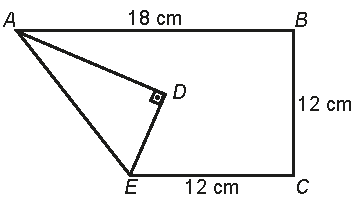
\includegraphics[width=0.95\linewidth]{Q166.pdf}
    %\caption{}
    \label{fig:q166}
\end{figure}

Após essa primeira dobradura, a medida do segmento AE é

A) $ 2\sqrt{22} cm $.

B) $ 6\sqrt{3} cm $.

C) $ 12 cm $.

D) $ 6\sqrt{5} cm $.

E) $ 12\sqrt{2} cm $.

\textbf{Resolução}

É muito óbvio a aplicação direta do Teorema de Pitágoras:

Um dos catetos será a diferença entre o lado maior do retângulo e o início da dobra, ou seja $ 18cm - 12cm = 6cm $ e o outro $12 cm$ correspondentes ao lado menor do retângulo


\tikzset{every picture/.style={line width=5pt}} %set default line width to 0.75pt        

\noindent \resizebox{.5\textwidth}{!}{
    
    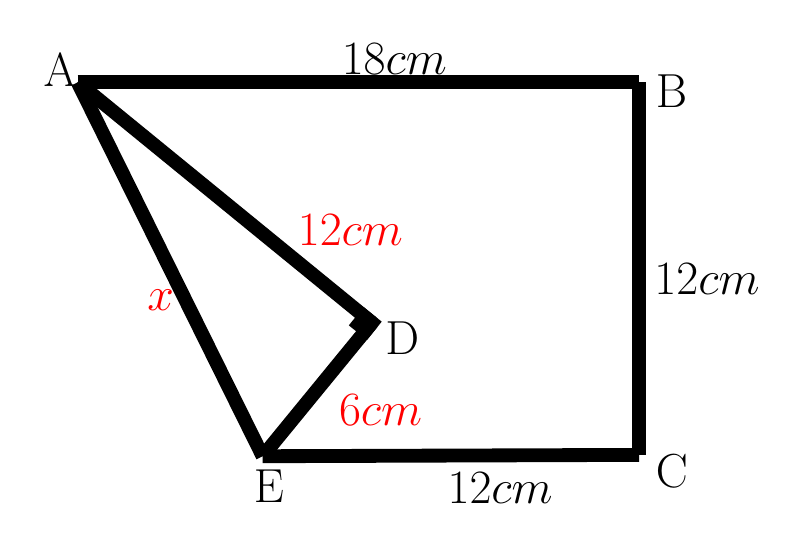
\begin{tikzpicture}[x=0.75pt,y=0.75pt,yscale=-.5,xscale=.5]
    \draw    (61.5,31) -- (602.5,31) ;
    \draw    (602.5,31) -- (602.5,390) ;
    \draw    (239.8,391.29) -- (602.5,390) ;
    \draw    (61.5,31) -- (239.8,391.29) ;
    \draw    (345.13,262.63) -- (239.8,391.29) ;
    \draw    (61.5,31) -- (345.13,262.63) ;
    \draw   (338,256.91) -- (345.13,262.63) -- (339.32,269.88) -- (332.18,264.16) -- cycle ;
    \draw  [fill={rgb, 255:red, 0; green, 0; blue, 0 }  ,fill opacity=1 ] (337.06,263.39) .. controls (337.06,262.51) and (337.78,261.8) .. (338.66,261.8) .. controls (339.54,261.8) and (340.25,262.51) .. (340.25,263.39) .. controls (340.25,264.27) and (339.54,264.99) .. (338.66,264.99) .. controls (337.78,264.99) and (337.06,264.27) .. (337.06,263.39) -- cycle ;
    
    \draw (20,-5) node [anchor=north west][inner sep=0.75pt]  [font=\LARGE] [align=left] {A};
    \draw (610,14.67) node [anchor=north west][inner sep=0.75pt]  [font=\LARGE] [align=left] {B};
    \draw (610,381.33) node [anchor=north west][inner sep=0.75pt]  [font=\LARGE] [align=left] {C};
    \draw (349.33,252.67) node [anchor=north west][inner sep=0.75pt]  [font=\LARGE] [align=left] {D};
    \draw (222.67,395.33) node [anchor=north west][inner sep=0.75pt]  [font=\LARGE] [align=left] {E};
    
    \draw (307.33,-15) node [anchor=north west][inner sep=0.75pt]  [font=\LARGE]  {$18cm$};
    \draw (608.67,197.4) node [anchor=north west][inner sep=0.75pt]  [font=\LARGE]  {$12cm$};
    \draw (409.33,398.73) node [anchor=north west][inner sep=0.75pt]  [font=\LARGE]  {$12cm$};
    
    \draw (304.67,323.4) node [color=red,anchor=north west][inner sep=0.75pt]  [font=\LARGE]  {$6cm$};
    \draw (265,150) node [color=red,anchor=north west][inner sep=0.75pt]  [font=\LARGE]  {$12cm$};    
    \draw (120,222.73) node [color=red,anchor=north west][inner sep=0.75pt]  [font=\LARGE]  {$x$};
    
    \end{tikzpicture}
    
}

Disso temos, por Pitágoras:


\begin{eqnarray*}
    x^2 &=& 12^2 + 6^2 \\
        &=& 144 + 36 \\
        &=& 180 \\
        & & \\
    x^2 &=& 180 \\  
    x   &=& \sqrt{180} \\  
        &=& \sqrt{2^2 \cdot 3^2 \cdot 5}\\  
        &=& 2 \cdot 3 \cdot \sqrt{5}\\  
    x   &=& 6 \sqrt{5} \approx 6 \cdot 2,23 \approx  13,38
\end{eqnarray*}

\textbf{Rascunho}

\getprime{200}%

\opmul[decimalsepsymbol={,},displayintermediary=all,voperation=top]{12}{12}\flexquad{3}
\primedecomp[voperation=top]{180}
\opmul[decimalsepsymbol={,},displayintermediary=all,voperation=top]{2.23}{6}\flexquad{3}


\begin{center}
    \href{https://youtu.be/}{
        \qrcode{https://youtu.be/}
    }\\
    Resolução: \url{https://youtu.be/}
\end{center}
